\begin{frame}
  \frametitle{Born-Oppenheimer Molecular Dynamics (BOMD)}
  \begin{itemize}
    \item Problem: Klassische Kraftfelder können keine chem. Reaktionen beschreiben $\rightarrow$ Quantenmechanik benötigt!
    \item Kräfte- und Energieberechnung mittels \textbf{semi-empirischer Methoden} anstatt des Lennard-Jones-Potentials möglich
    \item Anwendung: Modellierung einer Diels-Alder-Reaktion
    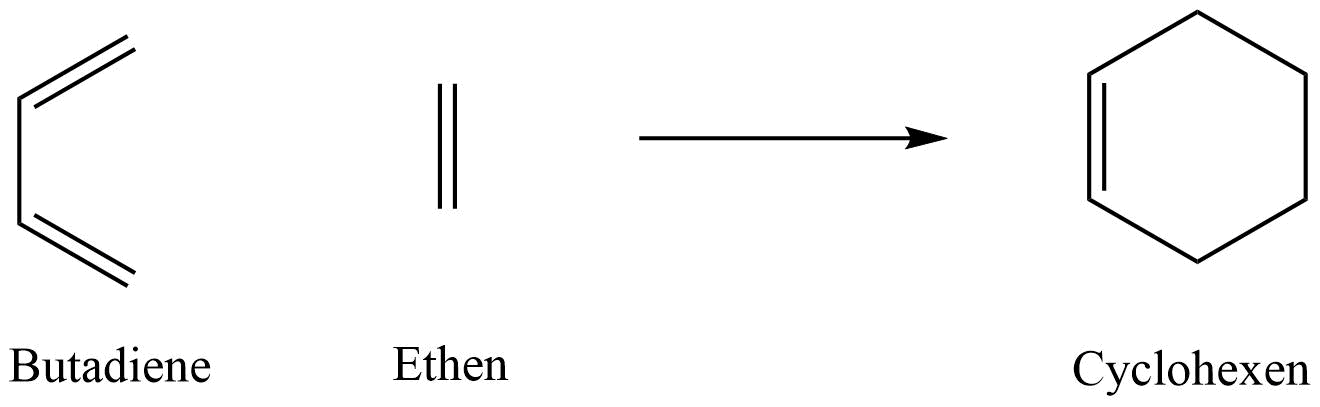
\includegraphics[scale=0.15]{DielsAlder.png}
    \item Kollision der beiden Moleküle mit verschiedenen Anfangsgeschwindigkeiten
    \item Minimale Geschwindigkeit bestimmen, bei der die Reaktionsbarriere überwunden wird $\rightarrow$ Reaktionsbarriere abschätzen
  \end{itemize}
\end{frame}
